\documentclass[11pt]{article}
\usepackage[pdftex]{graphicx}
\usepackage[explicit]{titlesec}
\usepackage[OT1]{fontenc}
\usepackage[most]{tcolorbox}
\usepackage[final]{pdfpages}
\usepackage[colorlinks=true, urlcolor=cyan, hyperfootnotes=false]{hyperref}
\usepackage{fullpage, graphicx, psfrag, url, caption, authblk, amsfonts, amsmath, amssymb, float, fancyhdr, multicol, cmbright, xcolor, amsthm, gensymb, physics}

\fancypagestyle{pages}{
	%Headers
	\fancyhead[L]{Physics 7A, Summer 2024 \\ Section 103}
	%\fancyhead[C]{\thepage}
	\fancyhead[R]{Discussion 12 \\ July 18}
\renewcommand{\headrulewidth}{0pt}
	%Footers
	%\fancyfoot[L]{}
	\fancyfoot[C]{}
	\fancyfoot[R]{\thepage}
\renewcommand{\footrulewidth}{0pt}
}

\newcommand\blfootnote[1]{
    \begingroup
    \renewcommand\thefootnote{}\footnote{#1}
    \addtocounter{footnote}{-1}
    \endgroup
}

\newcommand{\fig}[4]{
    \begin{figure}[H]
        \centering
        \includegraphics[scale={#3}, angle={#4}]{#1}
        \caption{#2}
        \label{exp4fit}
    \end{figure}
}

\newtheoremstyle{gangnamstyle}{}{}{}{}{\sffamily\bfseries}{.}{ }{}
\tcolorboxenvironment{definition}{boxrule=0pt,boxsep=0pt,colback={blue!10},left=8pt,right=8pt,enhanced jigsaw, borderline west={2pt}{0pt}{blue},sharp corners,before skip=10pt,after skip=10pt,breakable}
\tcolorboxenvironment{example}{boxrule=0pt,boxsep=0pt,colback={orange!10},left=8pt,right=8pt,enhanced jigsaw, borderline west={2pt}{0pt}{orange},sharp corners,before skip=10pt,after skip=10pt,breakable}
\tcolorboxenvironment{problem}{boxrule=0pt,boxsep=0pt,colback={cyan!10},left=8pt,right=8pt,enhanced jigsaw, borderline west={2pt}{0pt}{cyan},sharp corners,before skip=10pt,after skip=10pt,breakable}
\theoremstyle{gangnamstyle}{\newtheorem{definition}{Definition}[]}
\theoremstyle{gangnamstyle}{\newtheorem{example}{Example}[]}
\theoremstyle{gangnamstyle}{\newtheorem{problem}{Problem}[]}

\headheight=0pt
\footskip=0pt
\setlength{\oddsidemargin}{0 in}
\setlength{\evensidemargin}{0 in}
\setlength{\topmargin}{-0.5 in}
\setlength{\textwidth}{6.5 in}
\setlength{\textheight}{8.5 in}
\setlength{\headsep}{0.75 in}
\setlength{\parindent}{0 in}
\setlength{\parskip}{0.1 in}

\begin{document}
\normalfont
\pagestyle{pages}

% Begin Document

\begin{center}
\vspace{3in}
{\Large Discussion 12 } \\ [0.05in]
Rotational Motion \\ [-0.5in]
\end{center}

\section*{Topics}
Angular Position, Velocity, and Acceleration. 

Torque, Moment of Inertia, and Rotational Kinetic Energy. 

\section{Review}

\subsection{Cross Products}

Please refer to sections 2.2, 2.3 of these \href{https://bcourses.berkeley.edu/courses/1535243/files/folder/Section/103/Notes?preview=89181658}{Notes} for a comprehensive review on cross products. 

The \textbf{Cross Product} of two vectors is a vector quantity that is perpendicular to both initial vectors. 

For vectors $\Vec{A}$ and $\Vec{B}$, 
\[ \Vec{A} = A_x\Hat{x} + A_y\Hat{y} + A_z\Hat{z} \]
\[ \Vec{B} = B_x\Hat{x} + B_y\Hat{y} + B_z\Hat{z} \]

Their cross product is defined as the $3 \times 3$ determinant
\[ \Vec{A} \times \Vec{B} = 
\begin{vmatrix}
\Hat{x} & \Hat{y} & \Hat{z} \\
A_x & A_y & A_z \\
B_x & B_y & B_z
\end{vmatrix} \]
Or alternatively, 
\[ \Vec{A} \times \Vec{B} = 
\begin{vmatrix}
A_y & A_z \\
B_y & B_z
\end{vmatrix} \Hat{x}
- 
\begin{vmatrix}
A_x & A_z \\
B_x & B_z
\end{vmatrix} \Hat{y}
+ 
\begin{vmatrix}
A_x & A_y \\
B_x & B_y
\end{vmatrix} \Hat{z} \]
Expanding the $2 \times 2$ determinants, 
\[ \Vec{A} \times \Vec{B} = (A_yB_z - A_zB_y) \Hat{x} - (A_xB_z - A_zB_x) \Hat{y} + (A_xB_y - A_yB_x) \Hat{z} \]

\fig{../notes/figs/n0/times.png}{Cross Product and the Right-Hand Rule}{0.35}{0} 

The cross product has the following properties: 

The cross product, $\Vec{A} \times \Vec{B}$, is perpendicular to both $\Vec{A}$ and $\Vec{B}$. 
\[ (\Vec{A} \times \Vec{B}) \perp \Vec{A} \]
\[ (\Vec{A} \times \Vec{B}) \perp \Vec{B} \]

The magnitude of a cross product equals to
\[ |\Vec{A} \times \Vec{B}| = AB \sin\theta \]
Where $A$, $B$ are the magnitudes of the vectors, and $\theta$ is the angle between the $\Vec{A}$, $\Vec{B}$ vectors. \\

The direction of the resulting vector is given by the Right-Hand Rule, as illustrated in the figure above. To find the direction of $(\Vec{A} \times \Vec{B})$, 
\begin{enumerate}
\item Align the palm of your right hand in the direction of $\Vec{A}$ (The first vector),
\item Bend your four fingers toward the direction of $\Vec{B}$ (The second vector),
\item Then your thumb would naturally point toward the direction of the resultant vector $(\Vec{A} \times \Vec{B})$. 
\end{enumerate}
\textit{If you reverse the order of steps 1 and 2, or if you use the left hand, your answer will end up in the opposite direction. (Sorry lefties!)} \\

The cross product of a vector with itself is the zero vector. In fact, because $\sin(0 \degree) = \sin(180 \degree) = 0$, the cross product of all parallel/antiparallel vectors are zero. 
\[ \Vec{A} \times \Vec{A} = \Vec{0} \]
The cross product is anti-commutative and distributive. 
\[ \Vec{A} \times \Vec{B} = - \Vec{B} \times \Vec{A} \]
\[ \Vec{A} \times (\Vec{B} + \Vec{C}) = \Vec{A} \times \Vec{B} + \Vec{A} \times \Vec{C} \]

We can also apply the Product Rule when taking the derivative of a cross product. 
\[ \frac{d}{dt}(\Vec{A} \times \Vec{B}) = \frac{d\Vec{A}}{dt} \times \Vec{B} + \Vec{A} \times \frac{d\Vec{B}}{dt} \]

\subsection{Angular Position, Velocity and Acceleration}

The \textbf{Angular Position} $\theta$, usually measured in terms of radians, is the angle at which an object is oriented with respect to some reference position. 
\fig{figs/0718/radian.png}{Angular Position}{0.65}{0}
By the arc length formula, 
\[ s = r\theta \]
Differentiate this equation with respect to time. 
\[ v = r\omega \]
\[ a = r\alpha \]
Where $v$, $a$ are the speed and acceleration in the tangential direction, $\omega$ is the angular velocity ($rad/s$), $\alpha$ is the angular acceleration ($rad/s^2$). 

When the angular acceleration $\alpha$ is constant, these angular quantities obey the \textbf{Kinematics Equations}, just like their translational counterparts. 
\[ \theta = \theta_0 + \omega_0 t + \frac{1}{2} \alpha t^2 \]
\[ \omega = \omega_0 + \alpha t \]
\[ \omega^2 = \omega_0^2 + 2\alpha(\theta - \theta_0) \]
\[ \omega_{avg} = \frac{1}{2}(\omega + \omega_0) \]


$\Vec{\omega}$ and $\Vec{\alpha}$ are \textbf{vectorial quantities}, and they obey all rules and properties we've previously discussed regarding vectors. The directions of the vectors are defined such that a Counterclockwise rotation in the $x$-$y$ plane has the $\Vec{\omega}$ vector point in the $+z$ direction. This is also obtained from the Right-Hand Rule. 

\fig{figs/0718/rh-rule.png}{Right-Hand Rule when Obtaining Rotational Vectors}{0.5}{0}

\fig{figs/0718/rotations.png}{Angular Position is not a Vector!}{0.65}{0}

\textbf{However, the angular position $\theta$ is not a vector! Vector additions are commutative,}
\[ \Vec{A} + \Vec{B} = \Vec{B} + \Vec{A} \]
\textbf{But the addition of angular position is not commutative, as illustrated in the drawing above. }

\pagebreak

\subsection{Inertia, Torque, and Momentum}

The \textbf{Moment of Inertia}, $I$, is the rotational analogy of mass. It is the tendency of an object to resist an applied torque. It is defined as

Discrete objects:
\[ I = \sum m_i r_{i \perp}^2 \]
\textit{(The moment of inertia of a point mass is thus)}
\[ I = mr_\perp^2 \]
Continuous objects:
\[ I = \int r_{\perp}^2 \ dm \]
The perpendicular symbol $\perp$ means that only components that are perpendicular to the rotational axis contribute to the moment of inertia. For example, say you rotate a pencil with respect to the vertical, if you hold the pencil upright, it takes little effort (lower moment of inertia) to spin the pencil; if the pencil was positioned horizontally, it takes more effort (higher moment of inertia) to spin the pencil. 

The \textbf{Parallel Axis Theorem} states that
\[ I = I_{CM} + MR^2 \]
Where $I$ is the momentum of inertia viewed from an arbitrary point, $I_{CM}$ is the moment of inertia at the center of mass, $M$ is the total mass of the object, and $R$ is the distance between CM and the arbitrary point. \\

The \textbf{Torque}, $\Vec{\tau}$, is the rotational analogy of the linear force. A torque causes an angular acceleration. The rotational version of Newton's Second Law says, 
\[ \sum\Vec{\tau} = I \Vec{\alpha} \]
Similarly, the \textbf{Angular Momentum}, $\Vec{L}$ is the rotational analogy of the linear momentum. 
\[ \Vec{L} = I\Vec{\omega} \]
Indeed, the momentum form of Newton's Second Law also manifests in rotational motion. 
\[ \sum\Vec{\tau} = \frac{d\Vec{L}}{dt} \]

\pagebreak

\subsection{Relationship Between Linear and Angular Quantities}

When we relate the linear and rotational \textbf{Kinematic Quantities}, the tangential velocity and acceleration obey the arc length formulas, 
\[ v_T = r\omega \]
\[ a_T = r\alpha \]

\fig{figs/0718/conversions.jpeg}{Counterclockwise Rotation of a Disk in the $x$-$y$ plane}{0.15}{0}

And applying the Right-Hand Rule on the rotating disk above, we can see that the directions of the vector quantities must obey
\[ \Vec{v}_T = \Vec{\omega} \times \Vec{r} \]
\[ \Vec{a}_T = \Vec{\alpha} \times \Vec{r} \]

For the radial acceleration from Uniform Circular Motion, 
\[ a_R = \frac{v_T^2}{r} = v_T\omega \]
It follows that 
\[ \Vec{a}_R = \Vec{\omega} \times \Vec{v} \]

\pagebreak

In fact, these cross products hold even for rotations not centered at the origin, like the example below, where $|\Vec{\omega} \times \Vec{r}| = \rho \omega$. 
\fig{figs/0718/particle.png}{A Rotating Particle}{0.6}{0}

When we convert \textbf{Dynamic Quantities}, the relationships are
\[ \Vec{\tau} = \Vec{r} \times \Vec{F} \]
And
\[ \Vec{L} = \Vec{r} \times \Vec{p} \]
As shown in the figure below. 

\fig{figs/0718/momentum.png}{Relating Linear and Angular Momentum}{0.4}{0}

\pagebreak

\subsection{Conservation Laws}

When an object rotates, it carries \textbf{Rotational Kinetic Energy} about the axis of rotation. 
\[ K = \frac{1}{2}I\Vec{\omega}^2 \]
For an object that undergoes both translational and rotational motion (such as Earth orbiting the sun while also spinning about its own axis), its total kinetic energy is
\[ K = \frac{1}{2}M\Vec{V}_{CM}^2 + \frac{1}{2}I_{CM}\Vec{\omega}^2 \]
Where $M$ is the total mass of the object, $\Vec{V}_{CM}$ is the velocity of its center of mass, $I_{CM}$ is the inertia with respect to the CM, and $\Vec{\omega}$ is the angular velocity as viewed from the CM. \\
The first term, $\frac{1}{2}M\Vec{V}_{CM}^2$, is the orbital kinetic energy, and the second term, $\frac{1}{2}I_{CM}\Vec{\omega}^2$, is the spin kinetic energy. \\

Lastly, under an absence of net external torque, the total angular momentum of a system is conserved. 
\[ \sum\Vec{\tau} = \Vec{0} \implies \Vec{L} = \text{constant} \]

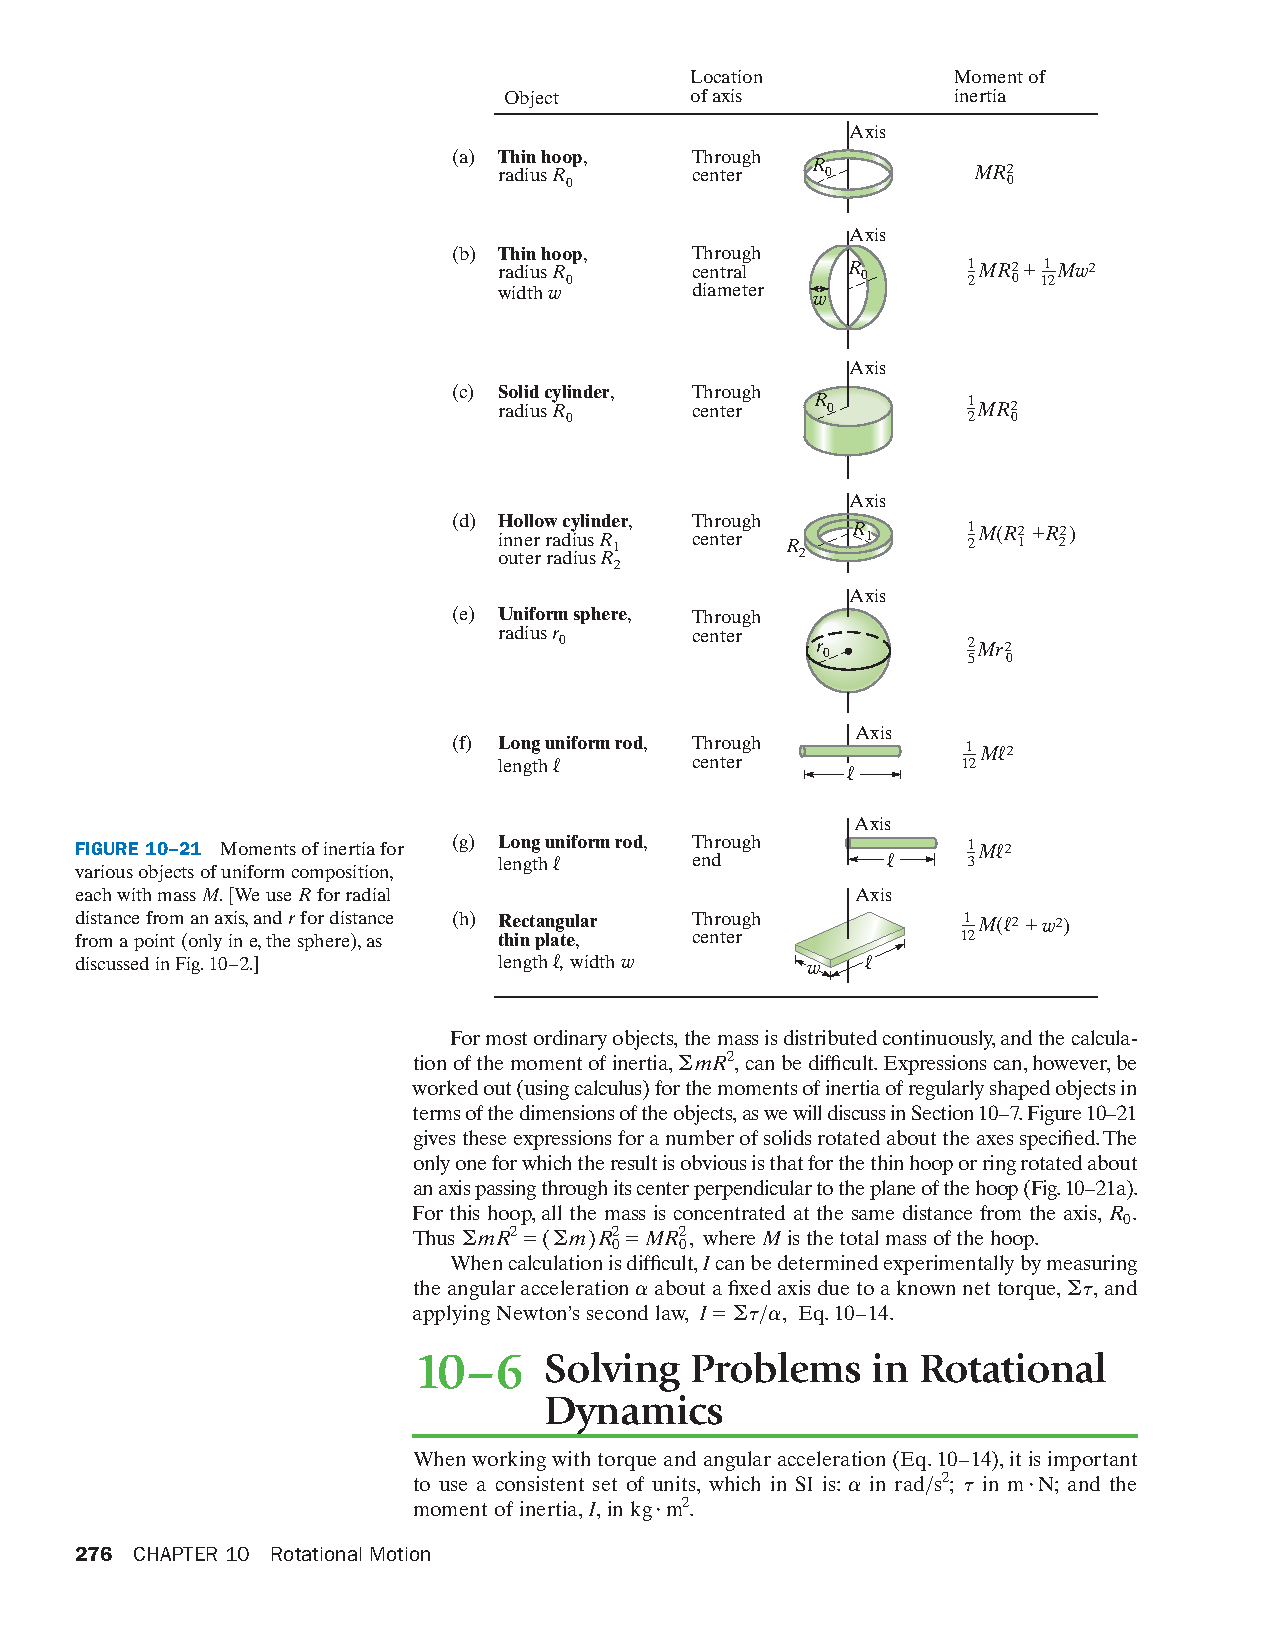
\includepdf[pages=-]{figs/0718/inertias.pdf}

\section{Rotational Motion}

\textbf{1.} \textit{Giancoli, Physics for Scientists and Engineers, Problem 10.51} \\
An Atwood machine consists of two masses, $m_A$ and $m_B$, connected by a massless inelastic cord that passes over a pulley free to rotate. The pulley is a solid cylinder of radius $R$ and moment of inertia $I$ about its axle. \\
(a) Determine the acceleration of each mass and the angular acceleration of the pulley. \\
(b) Would the accelerations be greater or less if we treat the pulley as massless and the moment of inertia of the pulley is ignored? \\
(c) Use the conservation of energy to solve part (a). \\
\textit{Hint: In part (a), the tensions $T_A$ and $T_B$ are not equal.}
\fig{figs/0718/g1051.png}{Giancoli, Problem 10.51}{0.6}{0}

\pagebreak

\textbf{2.} \textit{Giancoli, Physics for Scientists and Engineers, Problem 10.18} \\
The axle of a wheel is mounted on supports that rest on a rotating turntable as shown. The wheel has constant angular velocity $\omega_1 = 48 \ rad/s$ about its axle, and the turntable has constant angular velocity $\omega_1 = 35 \ rad/s$ about the vertical axis. (Note arrows showing these motions in the figure.) \\
(a) What are the directions of $\Vec{\omega}_1$ and $\Vec{\omega}_2$ at the instant shown? \\
(b) What is the total angular velocity of the wheel at the instant shown? Give the magnitude and direction. \\
(c) After the axis has rotated for $90 \degree$ (when the disk faces us), what is the total angular velocity of the wheel now? Again, give the magnitude and direction. 
\fig{figs/0718/g1018.png}{Giancoli, Problem 10.18}{0.6}{0}
\textit{Hopefully, this problem reminds you of Uniform Circular Motion where the linear velocity has constant magnitude and changing direction. Indeed, this is the rotational equivalent of UCM, called "Precession", and such an object that precesses is called a "Gyroscope". Precession is not covered in 7A, but if you are up for a challenge, you should try the last problem in the worksheet.}

\pagebreak

\textbf{3.} \textit{Giancoli, Physics for Scientists and Engineers, Problem 10.56} \\
A ball of mass $M$ and radius $r$ on the end of a thin massless rod is rotated in a horizontal circle of radius $R$ about an axis of rotation AB. \\
(a) Using the parallel-axis theorem and considering the finite radius of the ball, calculate the moment of inertia of the ball about AB. \\
(b) If we assume the mass of the ball to be concentrated at its center of mass, calculate its moment of inertia about AB. \\
The moment of inertial of the sphere about its center of mass is given by
\[ I = \frac{2}{5} Mr^2 \]
\fig{figs/0718/g56.png}{Giancoli, Problem 10.56}{0.6}{0}

\pagebreak

\textbf{4.} \textit{Giancoli, Physics for Scientists and Engineers, Problem 10.91} \\
What minimum horizontal force $F$ is needed to pull a wheel of radius $R$ and mass $M$ over a step of height $h$ as shown ($R > h$)? \\
(a) Assume the force is applied at the top edge as shown. \\
(b) Assume the force is applied instead at the wheel’s center.
\fig{figs/0718/g91.png}{Giancoli, Problem 10.91}{0.6}{0}

\pagebreak

\textbf{5.} \textit{Kleppner and Kolenkow, An Introduction to Mechanics, Problem 7.11} \\
A wheel is attached to a fixed shaft, and the system is free to rotate without friction. To measure the moment of inertia of the wheel–shaft system, a tape of negligible mass wrapped around the shaft is pulled with a known constant force $F$. When a length $L$ of tape has unwound, the system is rotating with angular speed $\omega$. Find the moment of inertia $I$ of the system.
\fig{figs/0718/kk711.png}{Kleppner and Kolenkow, Problem 7.11}{0.5}{0}

\pagebreak

\textbf{6.} \textit{Kleppner and Kolenkow, An Introduction to Mechanics, Problem 7.27} \\
A yo-yo of mass $M$ has an axle of radius $b$ and a spool of radius $R$. Its moment of inertia can be taken to be $I = \frac{1}{2}MR^2$. The yo-yo is placed upright on a table and the string is pulled with a horizontal force $F$ as shown. The coefficient of friction between the yo-yo and the table is $\mu$. What is the maximum value of $F$ for which the yo-yo will roll without slipping?
\fig{figs/0718/kk727.png}{Kleppner and Kolenkow, Problem 7.27}{0.5}{0}


\pagebreak

\textbf{7.} \textit{Kleppner and Kolenkow, An Introduction to Mechanics, Problem 7.37} \\
(a) A plank of length $2l$ and mass $M$ lies on a frictionless table. A ball of mass $m$ and speed $v_0$ strikes its end as shown. Find the final velocity of the ball, $v_f$, assuming that the collision is elastic and that $v_f$ is along the original line of motion. \\
\textit{Hint: For part (a), linear momentum, angular momentum, and kinetic energy are all conserved. For energy, consider the orbit (CM) and spin (rotational) kinetic energy of the rod. What is the initial angular momentum of the ball? }

(b) Find $v_f$ assuming that the stick is pivoted at the lower end. \\
\textit{Hint: For part (b), angular momentum and kinetic energy are conserved. Linear momentum is not conserved as the pivot exerts a force along the direction of the rod. }
\fig{figs/0718/kk737.png}{Kleppner and Kolenkow, Problem 7.37}{0.5}{0}
The momentum of inertia of this rod about its CM is
\[ I_{CM} = \frac{1}{3}ML^2 \]

\pagebreak

\begin{center}
(Blank Page)
\end{center}

\pagebreak

\textbf{8.} \textit{Morin, Introduction to Classical Mechanics, Problem 8.26} \\
A uniform stick of length $L$ is pivoted at its bottom end and is initially held vertical. It is given an infinitesimal kick, and it swings down around the pivot. After three-quarters of a turn (in the horizontal position shown in Fig. 8.39), the pivot is somehow vaporized, and the stick flies freely up in the air. \\
(a) What is the maximum height of the center of the stick in the resulting motion? \\
(b) At what angle is the stick tilted when the center reaches this maximum height? \\
\textit{Hint: When the stick enters free fall, there is no longer a torque when viewed from the center of mass, as gravity directly acts on its CM.}
\fig{figs/0718/m826.png}{Morin, Problem 8.26}{0.5}{0}
The momentum of inertia of this rod about its CM is
\[ I_{CM} = \frac{1}{12}ML^2 \]
The inertia about the pivot can be found using the Parallel Axis Theorem. 

\pagebreak

\textbf{9.} \textit{Kleppner and Kolenkow, An Introduction to Mechanics, Problem 7.12} \\
A pivoted beam has a mass $m_1$ suspended from one end and an Atwood’s machine suspended from the other. The frictionless pulley has negligible mass and dimension. Gravity is directed downward, and $m_2 > m_3$. Find a relation between $m_1$, $m_2$, $m_3$, $l_1$, and $l_2$ that will ensure that the beam has no tendency to rotate just after the masses are released. 
\fig{figs/0718/kk712.png}{Kleppner and Kolenkow, Problem 7.12}{0.6}{0}

\pagebreak

\section{The Gyroscope}
\textbf{10.} \textit{Kleppner and Kolenkow, An Introduction to Mechanics, Problem 8.1} \\
A thin hoop of mass $M$ and radius $R$ rolls without slipping about the $z$-axis. It is supported by an axle of length $R$ through its center, as shown. The hoop circles around the $z$-axis with angular speed $\Omega$. \\
(a) What is the total angular velocity, $\Vec{\omega}_{\text{total}}$, of the hoop? \\
(b) What is the angular momentum $\Vec{L}_{\text{total}}$ of the hoop? Is $\Vec{L}_{\text{total}}$ parallel to $\Vec{\omega}_{\text{total}}$? \\
The moment of inertia of a hoop for an axis along its diameter is $I = \frac{1}{2}MR^2$. \\
\textit{Hint: Consider both the orbit rotation ($\Vec{\Omega}$) and spin rotation ($\Vec{\omega}_s$). What is the magnitude of $\omega_s$ in terms of $\Omega$?}
\fig{figs/0718/kk81.png}{Kleppner and Kolenkow, Problem 8.1}{0.5}{0}

\end{document}
